\subsection{Il bilancio delle aziende}

\subsubsection{Sanitarie}

Il bilancio delle aziende sanitarie nasce per andare a capire la
situazione finanziaria, patrimoniale e reddituale dell'azienda
sanitaria.

Gli equilibri sono elementi di valutazione che ritroviamo nel bilancio,
il quale serve anche a valutare l'equilibrio economico,finanziario e
patrimoniale di una azienda.

\paragraph{Gli equilibri}

\begin{itemize}
\item
  \textbf{EQUILIBRIO FINANZIARIO E MONETARIO}: rappresenta le entrate e
  le uscite di moneta. L'erogazione di una prestazione (ad esempio un
  ricovero) genera un ritorno economico che si manifesta solitamente
  successivamente sotto il profilo finanziario (entrata di moneta). Non
  è detto che l'uscita di cassa sia nello stesso momento in cui utilizzo
  un bene. Quando acquisto io faccio una fattura che liquido
  successivamente. Nel lungo periodo i ricavi coincideranno con
  l'entrata e il flusso di cassa positivo. Il costo coinciderà con
  l'uscita di moneta. Quando acquisto un fattore produttivo ho un costo,
  la manifestazione finanziaria è il debito che nasce a seguito di quel
  costo.
\item
  \textbf{EQUILIBRIO REDDITUALE O ECONOMICO}: cattura i costi e i ricavi
  della gestione. Si va nelle aziende sanitarie a considerare i ricavi
  della gestione devono essere in grado di coprire i costi della
  gestione stessa. I ricavi fano riferimento alla cessione delle
  prestazioni sanitarie, i costi sono i consumi dei fattori produttivi
  che utilizzo per erogare la prestazione.
\end{itemize}

Entrambi gli equilibri sono rilevati dal bilancio di esercizio. Sono
importanti entrambi perchè i ricavi devono essere superiori ai costi
(composti da tanti elementi: personale, servizi, beni di consumo..). I
ricavi sono quello che entra all'azienda nel momento in cui si cede la
prestazione esternamente: faccio un ricovero e genero un DRG
(espressione e valore della prestazione prodotta) che mi da diritto al
rimborso da parte della regione, che però avviene successivamente quindi
sono due momenti separati.

Quindi il ricavo e il costo si trasformano successivamente in entrata di
moneta e uscita di moneta. Fanno entrambi parte della gestione ma sono
due momenti diversi. Non sempre i due equilibri coincidono perchè se io
non riscuotessi un DRG non raggiungo l'equilibrio. Il momento economico
è sulla produzione, il momento finanziario si muovono in maniera
parallela.

\begin{itemize}
\item
  \textbf{PATRIMONIO}: è l'insieme dei beni che sono a disposizione
  dell'azienda per perseguire l'equilibrio economico e finanziario nel
  lungo periodo. Es: se io cedo a terzi un' ala dell'ospedale (che mi
  permette di garantire prestazioni) ho un ricavo straordinario che
  potrebbe permettermi di raggiungere un equilibrio economico, mi pagano
  la vendita così ho entrata di moneta e raggiungo l'equilibrio
  finanziario MA se cedo un ala di ospedale è compromessa la possibilità
  di raggiungere l'equilibrio economico e finanziario nel lungo periodo.
  Per questo nel concetto di economicità c'è l'equilibrio dinamico nel
  tempo, non sono grandezze che devo valutare solo oggi ma mi devono
  dare delle indicazioni sulla capacità di perseguire gli obiettivi, che
  sono bisogni pubblici, nel lungo periodo.
\end{itemize}

Con la legge 502 del 1992 si è avviato il processo di aziendalizzazione,
questo ha portato una rivoluzione nei sistemi contabili e informativi
nell'azienda. Gli ospedali e le USL diventano aziende, e questo
determina una autonomia sotto il profilo contabile. Nasce un sistema
informativo che permette alle aziende di valutare il loro livello di
economicità attraverso il \emph{sistema della CONTABILITA ECONOMICO
PATRIMONIALE}. Questa è una rivoluzione sia sostanziale che formale, si
ha avuto un rinnovamento del sistema informativo (di cui il bilancio fa
parte). Il sistema di contabilità economico patrimoniale permette di
rilevare costi e ricavi (equilibrio economico), entrate e uscite
(equilibrio finanziario) e patrimonio: prima di questa modifica c'era la
cosidetta \emph{contabilità finanziaria} che andava solo a rilevare i
flussi di cassa, cioè solo le entrate e le uscite. Ci doveva essere un
equilibrio tra entrate e uscite (se spendo cento deve entrarmi cento):
queste informazioni sono però insufficienti per raggiungere il principio
di economicità, il sistema non rendeva disponibiliti tutte le
informazioni utili, oggi invece si con una conoscenza a 360 gradi sulle
attività e le risultanze dell'attività dell'azienda.

Il motivo per cui prima c'era solo l'equilibrio finanziario prima della
legge del 1992 è che questo equilibrio era espressione di un iter
giuridico e amministrativo precedente alla spesa. Le risorse a
disposizione della pubblica amministrazione derivano dalle tasse, quindi
si riteneva giusto dare a priori una indicazione di come queste entrate
poi potevano essere spese a livello regionale. Il bilancio andava a
valutava come queste entrate venivano spese, non calcolava costi e
ricavi. I bilanci si focalizzavano sull'aspetto preventivo (bilancio
quadriennale e annuale preventivo),con questo si dava evidenza di come
le entrate sarebbero poi state utilizzate. C'era poi un rendiconto solo
finanziario per specificare informazioni aggiuntive sulle entrate e le
uscite, ma tutto ciò aveva una rilevanza minore rispetto a oggi poichè
seguiva una logica autorizzativa, le attività dovevano essere approvate
da un ente superiore. Aveva un focus ex ante la gestione, i bilanci sono
redatti al 31/12 dell'anno di riferimento.

I comuni, lo stato e le regioni funzionano ancora con questa logica: i
problemi sono legati al fatto che i vincoli non venivano rispettati e
che la contabilità finanziaria non da informazioni utili su come
valutare il principio dell'economicità e come sta andando la gestione.
Con la legge del 1992 si supera la logica finanziaria.

Secondo il nuovo ordinamento si seguono gli articoli del codice civile,
cioè quelli seguiti anche dalle aziende private; resta il bilancio
economico pluriennale di previsione basati però sulla logica economica e
non più finanziaria, perdono la funzione autorizzativa ma svolgono un
ruolo perlopiù gestionale utilizzati fare programmazione. Bisogna dare
comunque evidenza a priori su come l'ospedale investe le risorse ma si
fa per un motivo gestionale e non più per una logica autorizzativa.
Vengono introdotti meccanismi di rilevazione di costi e ricavi più
complessi attraverso la contabilità analitica, ha il focus sui centri di
costo che costituiscono l'azienda. I bilanci devono essere resi pubblici
pubblicati sul sito internet delle aziende ospedaliere alla voce
trasparenza. Dopo un periodo di passaggio dal 1995 la contabilità
finanziaria è stata definitivamente soppressa e ad oggi è in vigore solo
la contabilità economico patrimoniale.

\paragraph{Gli strumenti sotto il profilo del sistema informativo di una azienda sanitaria (ASL e AO/AOU)}

\begin{itemize}
\item
  BILANCIO PLURIENNALE solitamente di tre anni, redatto tutti gli anni
  dove si dicono le politiche e le risorse impiegate per raggiungere gli
  obiettivi di lungo periodo, fortemente legato al piano nazionale e
  regionale e alle loro linee guida per garantire la massima coerenza.
\item
  BILANCIO ANNUALE DI PREVISIONE: espone il programma che verrà svolto,
  i ricavi e i costi che si prevedono. Strumento di programmazione
  redatto a priori prima del 31\textbackslash{}12.
\end{itemize}

Si utilizza la CONTABILITA' GENERALE per alimentare i due bilanci
precedenti.

\begin{itemize}
\item
  BILANCIO DI ESERCIZIO: bilancio a consuntivo, cioè a posteriori (a
  differenza del pluriennale e dell'annuale che sono entrambi
  preventivi), mostra quali sono stati gli andamenti economici
  finanziari e patrimoniali dell'azienda di interesse. Ritroviamo in
  questo documenti tutti i precedenti equilibri.
\end{itemize}

Si parte dal piano sanitario nazionale, poi si stilano i piani regionali
sanitari (che hanno grande potere in sanità) per poi arrivare al piano
attuativo locale. Redige un bilancio pluriennale poi un bilancio
preventivo per un anno infine il rendiconto alla fine dell'anno. Questi
strumenti sono alimentati dalla contabilità generale, dalla contabilità
analitica e dal sistema budgettario (usato per redigere la parte a
preventivo).

\emph{\emph{CONTABILITA' GENERALE/ECONOMICO PATRIMONIALE}}: è un sistema
che mi permette in maniera cronologica di rilevare tutte le attività e
mi permette di capire la loro manifestazione reddituale o finanziaria
sul patrimonio e sull'azienda. Si esegue con la partita doppia (aspetto
economico e aspetto monetario) mentre prima la contabilità finanziaria
usava il metodo della partita semplice (alimentazione di un solo conto).
Questo tipo di contabilità permette di rilevare l'aspetto economico,
finanziario e patrimoniale. Arrivo ad un risultato che è il risultato
economico dell'esercizio (cioè dell'anno, generalmente corrisponde
all'anno solare: inizia il 1 gennaio e si conclude il 31 dicembre).

Riassumendo: I VALORI FINANZIARI SONO IL DENARO. IL CREDITO E IL DEBITO.
EROGO UNA PRESTAZIONE: CREDITO SOTTO IL PROFILO FINANZIARIO, RICAVO DAL
IL PUNTO DI VISTA ECONOMICO. ACQUISTO UN BENE: DEBITO E USCITA
FINANZIARIA, COSTO DAL PUNTO DI VISTA ECONOMICO. SONO ELEMENTI DISTINTI
CHE SI MUOVONO SU PIANI PARALLELI.

\paragraph{Il bilancio di esercizio}

Il bilancio si compone di due parti importanti: lo STATO PATRIMONIALE (valuta il patrimonio) e il CONTO ECONOMICO (valuta il reddito). Nel patrimonio vado a vedere la situazione finanziaria e patrimoniale, il
conto economico mi permette di capire l'equilibrio economico sotto il
profilo dei costi e dei ricavi. Il reddito è prodotto dalla gestione, mi
dice quanto ho prodotto in un arco temporale definito: quanti costi
(risorse impiegate) e quanti ricavi (quanto ho prodotto). Il reddito
generalmente è su base annuale, è calcolato alla fine dell'esercizio. Al
primo minuto del primo gennaio il risultato prodotto sarà zero, perchè
va a misurare quanto ho prodotto. Al punto zero non avrò prodotto. Il
patrimonio invece all'inizio dell'anno sarà già alimentato al contrario
del reddito, il quale si azzera ogni anno. E' la fotografia del numero
dei beni, debiti da incassare, crediti da riscuotere. Lo stato
patrimoniale è una grandezza macroeconomica che si influenza grazie agli
avvenimenti della gestione.

Redatto ad aprile dell'anno successivo. Si alimenta con la contabilità
generale (quella in partita doppia). E' un insieme di valori numerari
(finanziari e patrimoniali) e di valori economici (costi e ricavi). È
composto da 4 documenti fondamentali: stato patrimoniale (patrimonio e
entrate e uscite,fotografia di un dato momento dei beni dei crediti e
dei debiti), conto economico (rileva il momento economico, trovo costi e
ricavi), nota integrativa (informazioni che mi aiutano a leggere il
bilancio, è composta de decine di pagine) e relazione sulla gestione (lo
redige il direttore generale ed esprime qualitativamente gli obiettivi
raggiunti, le strategie da attuare in seguito e da informazioni
sull'andamento della gestione).

il bilancio ci da informazioni sull'utilizzo delle risorse, ha una
funzione informativa interna per chi deve gestire delle risorse
(direttore di struttura complessa o di dipartimento) e una funzione
informativa esterna (operatori del settore che esternamente hanno
interesse in quello che l'azienda fa ``stake holder'' o qualunque
cittadino se interessato). È uno strumento di controllo e di
responsabilizzazione, mi da una espressione di quale è il risultato
della gestione e quindi per controllare che si sia arrivati agli
obiettivi programmati. Ci permette di capire l'equilibrio economico che
prima del 1992 era impossibile da rilevare per assenza di un documento
che fornisse queste informazioni.

\paragraph{I principi di redazione del bilancio di esercizio}

Per redigere il bilancio ci sono dei principi contabili da seguire
durante la stesura, sono delle regole definite.

\begin{itemize}
\item
  PRUDENZA: i profitti non realizzati non devono essere contabilizzati
  mentre le perdite anche se non definitivamente realizzate devono
  essere imputate al bilancio.
\item
  CONTINUITA': le valutazioni devono essere effettuate nella prospettiva
  di continuità dell'attività, cioè sapendo che l'azienda perdurerà nel
  tempo.
\item
  COMPETENZA: si deve tenere conto degli oneri e dei proventi
  dell'esercizio indipendentemente dalla data di pagamento o incasso.
  Es: a gennaio ho un DRG per un ricovero che da diritto a rimborso di
  500 euro. Erogo il DRG il 10-12-2016 mandandolo alla regione, che
  verifica che tutto sia nella norma. Ad aprile 2017 la regione
  riconosce l'attività e ti da i 500 euro. Secondo questo principio i
  500 euro sono di competenza dell'anno 2016 perchè si tiene conto di
  quando la prestazione viene erogata e quindi di quando ho sostenuto il
  costo erogando la prestazione. Nella parte dello stato patrimoniale
  scriverò un credito di 500 euro. La manifestazione monetaria (entrata
  di moneta) avviene successivamente. Il DRG è una tariffa che copre i
  costi, cioè le risorse che io devo usare per erogare la prestazione.
  Non è detto che effettivamente ne spendi 500, dipende dall'efficienza
  interna della struttura. Sono tariffe stabilite su una previsione di
  costi per sostenere una attività. Il ricavo (500 euro) è fisso, nelle
  aziende sanitarie funziona cosi cioè le tariffe sono predefinite,
  esistono oltre 500 attività di DRG legate alle attività di ricovero
  definite a livello regionale.
\item
  VALUTAZIONE SEPARATE DI ELEMENTI ETEROGENEI: non si possono effettuare
  compensazioni tra valori anche se fanno riferimento allo stesso
  soggetto con il quale ho il debito o credito (es. la regione mi deve
  100 ma io devo 30 alla regione per altri motivi, devo riportare le due
  voci senza compensare).
\item
  COSTANZA NEI CRITERI DI VALUTAZIONE: i criteri di valutazione delle
  poste in bilancio devono essere uguali di anno in anno affinchè questi
  criteri siano paragonabili nel tempo e quindi si possano effettuare
  valutazioni su più anni.
\end{itemize}

TIPOLOGIA DI VALORI CHE ENTRANO NEL BILANCIO:

\begin{itemize}
\item
  \emph{dati oggettivi}: presentano una visione incontrovertibile degli
  eventi della gestione a cui si riferiscono (es: costi e ricavi).
\item
  \emph{dati stimati}: valori risultanti da valutazioni verificabili in
  futuro, ad oggi solo stimabile (es: svalutazione crediti o contenzioso
  tra azienda e privato, non so come andrà la causa ma devo mettere in
  conto un fondo per coprire le spese anche se ad oggi non so a quanto
  ammonta il costo da sostenere).
\item
  \emph{dati congetturati}: dati derivanti da valutazioni congrue (es:
  ammortamenti). I fattori produttivi impiegati da un'azienda sono di
  diversa natura: forza lavoro, farmaci, macchinari. Se il farmaco lo
  uso in maniera immediata, al contrario un macchinario è uno strumento
  che mi permette di svolgere l'attività per un periodo lungo di tempo,
  continuerò ad utilizzare questo fattore produttivo per un certo numero
  di anni. Come faccio a capire quanto di quel valore è da attribuire
  all'anno considerato? Distribuisco un valore di un costo strategico
  pluriennale al singolo esercizio, nella pratica si prende il costo
  della tac (es 10.000 euro) e si divide per la vita utile dello
  strumento (es. 10 anni). E' un dato congetturato perchè non è detto
  che lo utilizzi davvero per quella durata, quindi è una stima. Mi
  permette di spalmare il costo per un arco temporale più ampio. Non
  potrò mai verificare se a posteriori ho attribuito la stima giusta. Se
  mi si rompesse la tac al terzo anno, avrei dovuto mettere 5000 e 5000
  i primi due anni, ma questo non era prevedibile. L'ammortamento è la
  quota di costo che un bene pluriennale cede al singolo esercizio. In
  realtà si tiene anche conto del fatto che se acquisto un bene il
  valore va aggiunto al patrimonio (TAC +10.000 che ogni anno va a
  ridursi). Se si rompe una tac ad esempio elimino il bene dal
  patrimonio e aggiungo un costo per il restante che è rimasto rispetto
  all'ammortamento (es. 8000 euro). Se all'undicesimo anno la tac
  funziona ancora ed è finito l'ammortamento, continuo ad usarla ma non
  ho più quote di ammortamento. Avrò un valore pari a zero nel
  patrimonio perchè ho usato tutto il suo fattore produttivo. Quando
  finisco di ammortizzarlo non posso continuare a riportare i costi e
  neanche il valore come attivo. Se cedo il bene (vendita) aggiungo il
  ricavo per cessione nel bilancio.
\end{itemize}

Riassumendo, il reddito di esercizio è il risultato economico d'impresa
astrattamento attribuito a un determinato periodo amministrativo. Alla
sua formazione concorrono valori certi, stime e congetture. Fa
riferimento all'anno solare, calcolo il risultato in un arco di tempo
definitivo e si può calcolare in diversi modi. Vediamo solo quello
derivante dal conto economico (reddituale).

\subsubsection{Schema di sintesi del conto economico}

Valore della produzione -- costi della produzione = differenza tra
valore e costi della produzione

+\textbackslash{}- proventi e oneri finanziari

+\textbackslash{}- rettifiche di valore di attività finanziarie

+\textbackslash{}- proventi e oneri straordinari

RISULTATO DI ESERCIZIO = ricavi -- costi (consumi, fondi, ammortamento)
= \emph{utile} (se è positivo, cioè se i ricavi sono superiori ai costi)
o \emph{perdita} (se è negativo, cioè se ho più costi che ricavi).

Aver prodotto un utile o una perdita che significato ha in sanità? In
una azienda privata il ricavo deve essere maggiore dei costi mentre in
una attività pubblica questo non è l'obiettivo principale. L'utile non è
il criterio principale su cui valutare la qualità del servizio
(soddisfazione del personale, reputazione, qualità delle cure offerte
etc). Per una azienda privata non bisogna avere costi = ricavi ma ricavi
\textgreater{} costi. Quindi il bilancio di esercizio ci da una mano a
prendere decisioni ma la valutazione positiva non deriva solo dall'avere
ricavi maggiori dei costi perchè l'obiettivo è soddisfare la salute dei
cittadini. Da solo non ci da informazioni su altre cose tipo la
soddisfazione dei ricoverati etc.

Ricavi di una azienda (valore di produzione): soldi dalla regione, dallo
stato, tariffe drg, ricavi da gestione finanziaria,ticket cioè
partecipazione del privato alla spesa, altre entrate tipo funzioni
{[}FUNZIONI DI UNA AZIENDA SANITARIA: l'attività di ps non genera un DRG
in modo diretto ma lo stato e la regione lo riconoscono lo stesso, danno
un contributo in conto esercizio cioè una integrazione nei ricavi{]} più
altre forme di trasferimenti (la regione da dei ricavi per comprare un
macchinario particolare).

Costi (fattori produttivi impiegati): acquisto di beni servizi sanitari
e non sanitari, la voce grossa è il personale, suddivisione del
personale nelle diverse categorie, ammortamento (quote dei beni
pluriennali che costituiscono un costo, 1000 euro della tac, 5000
dell'ambulanza etc).

ESEMPIO: La asl ha l'obiettivo di garantire i LEA (livelli essenziali di
assistenza) ai cittadini che rientrano nel loro bacino di utenza, il
grosso deriva da trasferimenti di fondi regionali per garantire i LEA
perchè non hanno attività di ricovero che da DRG.

\begin{figure}[!ht]
\centering
	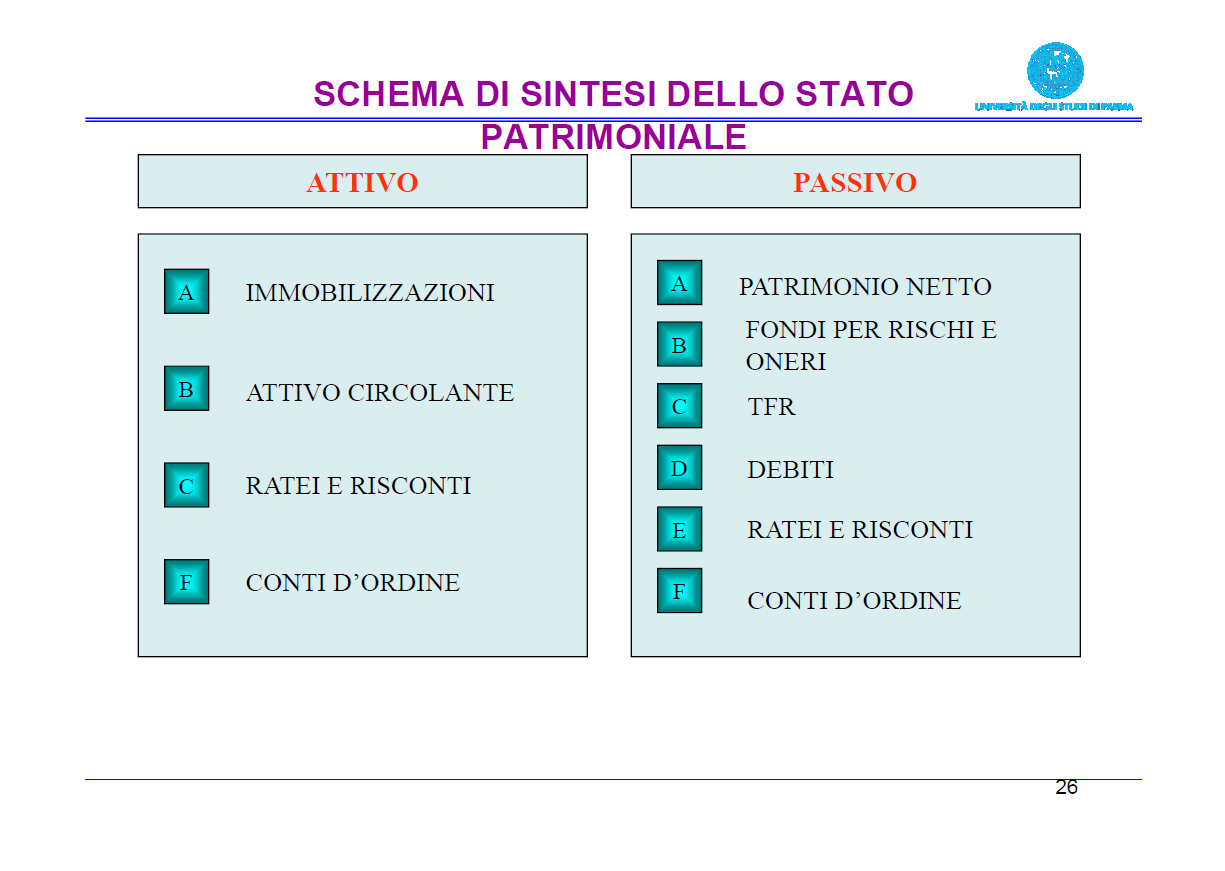
\includegraphics[width=0.7\textwidth]{15/image1.png}
	\end{figure}

\textbf{Immobilizzazioni}: tutti quei beni che hanno una valenza
pluriennale, possono essere tangibili o materiali (attrezzature varie)
oppure immateriali (ad esempio un brevetto) che posso ammortizzare (se
la durata è di venti anni lo ammortizzo per 20), oppure finanziari
(titoli) che vado a rivalutare ogni anno per capire il valore anno per
anno.

\textbf{Patrimonio netto}: nelle imprese private qui si trova il
capitale sociale, cioè le quote che i soci danno all'impresa. L'azienda
sanitaria è una derivazione della regione, quindi qui ci sono le risorse
finanziare e patrimoniali date all'azienda sanitaria dalla regione per
svolgere l'attività. Prende il nome di fondo di dotazione. Poi abbiamo
finanziamenti ricevuti dalla regione o stato per l'acquisto di
immobilizzazioni materiali o immateriali. Anche l'ultima riga del conto
economico va ad alimentare il patrimonio netto perchè il conto economico
ammonta a zero il primo gennaio ma questa non può essere un'informazione
che viene persa, quindi tutto il precedente viene messo nel passivo alla
voce utile (perdita) di esercizio nel patrimonio netto.

I debiti sono solitamente verso altre pubbliche amministrazioni, ratei e
risconti passivi per il principio della competenza economica.
